
\documentclass[a4paper,12pt,titlepage,final]{article}
% Language setting
% Replace `english' with e.g. `spanish' to change the document language
\usepackage[english, russian]{babel}

% Set page size and margins
% Replace `letterpaper' with `a4paper' for UK/EU standard size
\usepackage[letterpaper,top=2cm,bottom=2cm,left=3cm,right=3cm,marginparwidth=1.75cm]{geometry}
\usepackage{float}
% Useful packages
\usepackage{amsmath}
\usepackage{graphicx}
\usepackage[colorlinks=true, allcolors=blue]{hyperref}


\usepackage[T1,T2A]{fontenc}     % форматы шрифтов
\usepackage[utf8x]{inputenc}     % кодировка символов, используемая в данном файле
\usepackage{amsmath}      % для настройки размера полей
\usepackage{indentfirst}         % для отступа в первом абзаце секции
\begin{document}
\begin{titlepage}
    \begin{center}
    {\small \sc Московский Государственный Университет имени М. В. Ломоносова \\
    Факультет Вычислительной Математики и Кибернетики\\}
    \vfill
    
    {\large \bf Отчет по практическому заданию по курсу Распределённые системы\\}
    \end{center}
    \begin{flushright}
    \vfill {
    Воробьев Евгений\\
    428 группа\\
    }
    \end{flushright}
    \begin{center}
    \vfill
    {\small Москва\\2023}
    \end{center}
    \par
\end{titlepage}

% Автоматически генерируем оглавление на отдельной странице
\tableofcontents

\newpage
\section{Задача 1}
\begin{itemize}
\item Разработать программу которая реализует заданный алгоритм. 
\item Получить временную оценку работы алгоритма.
\end{itemize}

\subsection{Описание}\par
Все 25 процессов, находящихся на разных ЭВМ сети, одновременно выдали запрос на вход в критическую секцию. Реализовать программу, использующую древовидный маркерный алгоритм для прохождения всеми процессами критических секций.
Критическая секция:
\begin{verbatim}
<проверка наличия файла “critical.txt”>;
if (<файл “critical.txt” существует>) {
<сообщение об ошибке>;
<завершение работы программы>;
} else {
<создание файла “critical.txt”>;
sleep (<случайное время>);
<уничтожение файла “critical.txt”>;
}    
\end{verbatim}
Для передачи маркера использовать средства MPI.
Получить временную оценку работы алгоритма. Оценить сколько времени потребуется, если маркером владеет нулевой процесс. Время старта (время «разгона» после получения доступа к шине для передачи сообщения) равно 100, время передачи байта равно 1 (Ts=100,Tb=1). Процессорные операции, включая чтение из памяти и запись в память, считаются бесконечно быстрыми.
\subsection{Реализация}
Все процессы представлены в виде сбалансированного двоичного дерева. Каждый процесс имеет очередь запросов от себя и соседних процессов (1-го, 2-х или 3-х) и указатель в направлении владельца маркера.
Вход в критическую секцию
\begin{itemize}
    \item Если есть маркер, то процесс выполняет КС.
    \item Если нет маркера, то процесс:
    \begin{enumerate}
        \item помещает свой запрос в очередь запросов;
        \item посылает сообщение «ЗАПРОС» в направлении владельца маркера и ждет сообщений.
    \end{enumerate}
\end{itemize}
Процесс, не находящийся внутри КС должен реагировать на сообщения двух видов -«МАРКЕР» и «ЗАПРОС».
\begin{enumerate}
    \item Пришло сообщение «МАРКЕР»:
    \begin{itemize}
        \item М1. Взять 1-ый запрос из очереди и послать маркер его автору (концептуально, возможно себе).
        \item М2. Поменять значение указателя в сторону маркера.
        \item М3. Исключить запрос из очереди.
        \item М4. Если в очереди остались запросы, то послать сообщение «ЗАПРОС» в сторону маркера.
    \end{itemize}
    \item Пришло сообщение «ЗАПРОС»:
    \begin{itemize}
        \item Поместить запрос в очередь.
        \item Если нет маркера, то послать сообщение «ЗАПРОС» в сторону маркера, иначе (если есть маркер) - перейти на пункт М1.
    \end{itemize}
\end{enumerate}
\begin{figure}[h!]
  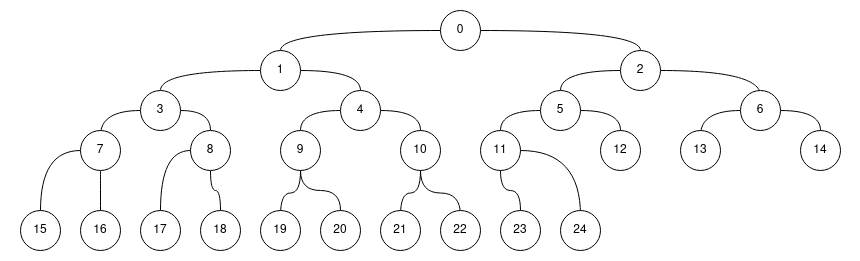
\includegraphics[width=1\linewidth]{marker.png}
  \caption{Схема системы передачи маркера}
  \label{fig:marker}
\end{figure}
\subsubsection{Запуск}
\begin{verbatim}
mpicc raymond.c -o raymond
mpiexec -np 25 --oversubscribe ./raymond
\end{verbatim}
или (безопаснее)
\begin{verbatim}
mpicc raymond.c -o raymond
mpiexec -np 25 --host=hostname:25 ./raymond
\end{verbatim}
\subsection{Временная оценка}
Cообщений передачи маркера с запросом – 21, маркера без запроса – 24, всего передач маркера – 45.\par
(Lz - запрос, Lm - маркер; считаем эти сообщения равными 1 байту)\par
Таким образом, (Ts+Tb*Lz)*21+(Ts+Tb*Lm)*45 = 6666.
\newpage
\section{Задача 2}
\subsection{Описание}
Доработать MPI-программу, реализованную в рамках курса “Суперкомпьютеры и параллельная обработка данных”. Добавить контрольные точки для продолжения работы программы в случае сбоя. Реализовать один из 3-х сценариев работы после сбоя: a) продолжить работу программы только на “исправных” процессах; б) вместо процессов, вышедших из строя, создать новые MPI-процессы, которые необходимо использовать для продолжения расчетов; в) при запуске программы на счет сразу запустить некоторое дополнительное количество MPI-процессов, которые использовать в случае сбоя.
\subsection{Реализация}
Была выбран стратегия продолжения работы на исправных процессах, которые бы продолжили работу.\par
Был добавлен \textit{error\_handler}, перераспределяющий процессы и переводящий их в точку начала прерванной итерации.
\begin{verbatim}
static void error_handler(MPI_Comm *comm, int *err, ...) {
    int len;
    char errstr[MPI_MAX_ERROR_STRING];

    rank_to_kill = -200;

    MPIX_Comm_shrink(*comm, &global_comm);
    
    MPI_Comm_rank(global_comm, &rank);
    MPI_Comm_size(global_comm, &size);
    
    MPI_Error_string(*err, errstr, &len);
    printf("Rank %d / %d: Notified of error %s\n", rank, size, errstr);
    
    MPI_Barrier(global_comm);
    eps = 0;
    //adaptive choice of rows(depends on process count)
    fst_r = ((rank * (N-2)) / size) + 1;
    lst_r = ((rank + 1) * (N-2)) / size + 1;
    cnt_r = lst_r - fst_r;
    printf("%d %d %d %d\n", rank, fst_r, lst_r, cnt_r);

    free(A);
    A = calloc((cnt_r + 2) * N2, sizeof(*A));

    longjmp(jbuf, 0);
}
\end{verbatim}
Были добавлены \textit{save\_checkpoint} и \textit{load\_checkpoint}, сохраняющие и загружающие текущее состояние данных. Данные хранятся в специальном файле состояния.
\begin{verbatim}
void save_checkpoint() {
    MPI_File file;
    MPI_File_open(global_comm, file_path, MPI_MODE_CREATE | MPI_MODE_WRONLY, MPI_INFO_NULL, &file);
    for (int i = 1; i <= cnt_r; i++) {
        MPI_File_write_at(file, sizeof(MPI_DOUBLE) * N2 * (fst_r + i), &A[i], N2, MPI_DOUBLE, MPI_STATUS_IGNORE);
    }
    MPI_Barrier(global_comm);
    MPI_File_close(&file);
}

void load_checkpoint() {
    free(A);
    A = calloc((cnt_r + 2) * N2, sizeof(*A));
    MPI_File file;
    MPI_File_open(global_comm, file_path, MPI_MODE_RDONLY, MPI_INFO_NULL, &file);
    for (int i = 1; i <= cnt_r; i++) {
        MPI_File_read_at(file, sizeof(MPI_DOUBLE) * N2 * (fst_r + i), &A[i], N2, MPI_DOUBLE, MPI_STATUS_IGNORE);
    }
    MPI_Barrier(global_comm);
    MPI_File_close(&file);
}
\end{verbatim}
\subsubsection{Запуск}
\begin{verbatim}
mpicc redb_3d_mpi_flthandle.c -o redb_3d_mpi_flthandle
mpiexec -np 4 --with-ft ulfm ./redb_3d_mpi_flthandle
\end{verbatim}
\section{Ссылки}
\begin{raggedright}
\begin{itemize}
\item \url{https://github.com/user-vo2/Skipod-tasks/tree/main/Skipod2}
\end{itemize}
\end{raggedright}
\end{document}